\section{Xây dựng bộ phân tích cú pháp}
\label{ch3:syntax-analysis}
Giai đoạn phân tích cú pháp là bước tiếp theo sau khi mã nguồn đã được chuyển đổi thành các từ tố bởi bộ phân tích từ vựng. Mục tiêu của giai đoạn này là xây dựng cây cú pháp trừu tượng (AST) để biểu diễn cấu trúc logic của mã nguồn, tạo nền tảng cho các giai đoạn phân tích ngữ nghĩa và thực thi sau này. 

    Việc xây dựng bộ phân tích cú pháp đòi hỏi một quy trình rõ ràng nhằm đảm bảo trình thông dịch có thể nhận diện đúng cú pháp và xử lý chính xác các câu lệnh phức tạp.

Trong ngôn ngữ Pandora, các loại câu lệnh như khai báo biến, biểu thức, câu lệnh điều khiển, và các cấu trúc phức tạp khác đóng vai trò quan trọng trong việc xây dựng logic của chương trình. Việc triển khai bộ phân tích cú pháp cho các câu lệnh này là một phần thiết yếu trong việc xây dựng trình thông dịch, giúp đảm bảo rằng tất cả các cấu trúc cú pháp được phân tích và xử lý đúng cách. Phần này sẽ giới thiệu cách thức bộ phân tích cú pháp hoạt động khi phân tích một số loại câu lệnh và biểu thức khác nhau.

\subsection{Câu lệnh}
    Quá trình phân tích cú pháp bắt đầu bằng việc nhận diện loại câu lệnh hiện tại. Điều này được thực hiện thông qua từ tố tiếp theo trong luồng đầu vào và được xử lý bởi hàm \kw{parse\_stmt}. Hàm này có nhiệm vụ phân loại câu lệnh dựa trên từ tố đầu tiên, từ đó chuyển hướng quá trình phân tích đến hàm phù hợp cho từng loại câu lệnh (ví dụ: khai báo biến, câu lệnh điều kiện, vòng lặp, v.v.).

\noindent \kw{src/parse/parser/stmt.rs}:
\begin{lstlisting}[]
pub fn parse_stmt(...) -> PResult<Box<Stmt>> {
    if self.token.is_keyword(Keyword::Set) {
        self.parse_stmt_var_decl()
    } else if self.token.is_keyword(Keyword::When) {
        self.parse_stmt_if()
    } else if self.token.kind == TokenKind::OpenDelim(Delimiter::Brace) {
        self.parse_stmt_block()
    } else if self.token.is_keyword(Keyword::During) {
        self.parse_stmt_while()
    } else if self.token.is_keyword(Keyword::For) {
        self.parse_stmt_for()
    } else if self.token.is_keyword(Keyword::Yeet) {
        self.parse_stmt_return()
    } else if self.token.kind == TokenKind::Semicolon {
        self.parse_stmt_empty()
    } else if self.token.is_keyword(Keyword::Fun) {
        self.parse_stmt_func_decl()
    } else if self.token.is_keyword(Keyword::Add) {
        self.parse_stmt_import()
    } else if self.token.is_keyword(Keyword::Br) {
        self.parse_stmt_break()
    } else if self.token.is_keyword(Keyword::Skip) {
        self.parse_stmt_continue()
    } else if self.token.can_begin_expr() {
        self.parse_stmt_expr()
    } else {
        let err = PError::ExpectedStatement {...};
        return Err(vec![err]);
    }
}
\end{lstlisting}

    Do có rất nhiều loại câu lệnh khác nhau, và quá trình xử lý mỗi loại câu lệnh tương đối phức tạp, ta sẽ chỉ trình bày chi tiết một vài loại câu lệnh tiêu biểu.

\noindent\textbf{Câu lệnh khai báo biến:}

    Cú pháp của câu lệnh khai báo biến được thể hiện thông qua biểu thức chính quy tại phần \textbf{\ref{ch2:decl_var_stmt}}. Câu lệnh khai báo biến được bắt đầu khi từ tố hiện tại là từ khóa \kw{set}. Việc phân tích câu lệnh này được thực hiện thông qua hàm \kw{parse\_stmt\_var\_decl} như sau:

\begin{lstlisting}[]
fn parse_stmt_var_decl(...) -> PResult<Box<Stmt>> {
    if !self.token.is_keyword(Keyword::Set) {
        let err = PError::ExpectedToken {...};
        return Err(vec![err]);
    }

    ...
    self.advance(); // 'set'

    let is_mut = if self.token.is_keyword(Keyword::Mut) {
        self.advance(); // 'mut'
        true
    } else {
        false
    };

    let ident = self.parse_ident()?;
    self.expect(TokenKind::Colon)?;
    self.advance(); // ':'
    let ty = self.parse_ty()?;

    let init = if self.token.kind == TokenKind::Eq {
        self.advance(); // expr
        Some(self.parse_expr()?)
    } else {
        None
    };

    self.expect(TokenKind::Semicolon)?;
    ...
    self.advance();

    let kind = if let Some(init) = init {
        LocalKind::Init(init)
    } else {
        LocalKind::Decl
    };

    ...
    let stmt = Box::new(Stmt {...});
    Ok(stmt)
}
\end{lstlisting}

    Cụ thể hàm \kw{parse\_stmt\_var\_decl} chịu trách nhiệm triển khai các bước phân tích cú pháp câu lệnh khai báo biến như sau:

\begin{itemize}
    \item \textbf{Xác định chế độ gán giá trị của biến}. Sau khi nhận diện từ khóa \kw{set}, trình thông dịch kiểm tra từ khóa bổ sung để xác định liệu biến được khai báo có thể thay đổi giá trị hay không. Nếu từ khóa \kw{mut} xuất hiện ngay sau \kw{set}, biến được đánh dấu là \kw{mutable} (có thể thay đổi giá trị). Ngược lại, biến sẽ là \kw{immutable} (không thể thay đổi giá trị).
    \item \textbf{Xác định tên biến}. Sau khi đã xác định được chế độ gán giá trị của biến, trình thông dịch sẽ đọc từ tố tiếp theo từ luồng đầu vào và kiểm tra để đảm bảo nó là một tên hợp lệ. Nếu tên không hợp lệ thì báo lỗi. 
    \item \textbf{Xác định kiểu dữ liệu của biến}. Sau khi xác định tên biến, trình thông dịch kiểm tra từ tố tiếp theo có phải là kí tự \kw{:} và xác định kiểu dữ liệu được chỉ định ngay sau nó bằng cách gọi hàm \kw{parse\_ty}. Nếu kiểu dữ liệu không hợp lệ thì báo lỗi. 
    \item \textbf{Kiểm tra, xử lý giá trị khởi tạo (nếu có) và phân loại}. Sau khi xác định kiểu dữ liệu, trình thông dịch sẽ kiểm tra từ tố tiếp theo. Nếu nó không phải là một dấu \kw{=} thì trình thông dịch xác định loại của câu lệnh khai báo là \kw{Declaration} (tức chỉ khai báo mà không gán giá trị). Ngược lại nếu nó là dấu '=' thì trình thông dịch sẽ xác định biểu thức khởi tạo ngay sau nó bằng cách gọi hàm \kw{parse\_expr} và xác định loại của câu lệnh khai báo là \kw{Initialization} (tức là câu lệnh khai báo có gán giá trị), nhưng nếu biểu thức này không hợp lệ thì báo lỗi. 
    \item \textbf{Đảm bảo câu lệnh kết thúc hợp lệ}. Câu lệnh khai báo kết thúc bởi một kí tự \kw{;}, do đó sau khi đã xác định xong các thành phần cơ bản của câu lệnh khai báo, trình thông dịch sẽ phải kiểm tra để đảm bảo tồn tại kí tự \kw{;} để kết thúc câu lệnh nếu như không tồn tại kí tự \kw{;} thì báo lỗi.
\end{itemize}


\noindent\textbf{Câu lệnh khai báo hàm:}

Cú pháp của câu lệnh khai báo biến được thể hiện thông qua biểu thức chính quy tại phần \textbf{\ref{ch2:decl_func_stmt}}. Câu lệnh khai báo hàm được bắt đầu khi từ tố hiện tại là từ khóa \kw{fun}. Việc phân tích câu lệnh này được thực hiện thông qua hàm \kw{parse\_stmt\_func\_decl} như sau:

\begin{lstlisting}[]
fn parse_stmt_func_decl(...) -> PResult<Box<Stmt>> {
    if !self.token.is_keyword(Keyword::Fun) {
        let err = PError::ExpectedToken {...};
        return Err(vec![err]);
    }
    ...
    self.advance();

    let sig = self.parse_stmt_func_sig()?;
    let body = self.parse_stmt()?;
    ...
    let stmt = Box::new(Stmt {...});
    Ok(stmt)
}
\end{lstlisting}

    Cụ thể hàm \kw{parse\_stmt\_func\_decl} chịu trách nhiệm triển khai các bước phân tích cú pháp câu lệnh khai báo hàm như sau:

\begin{itemize}
    \item \textbf{Xác định phần ký hiệu của hàm}. Sau khi nhận diện từ khóa \kw{fun}, trình thông dịch bắt đầu phân tích phần ký hiệu của hàm bằng cách gọi hàm \kw{parse\_stmt\_func\_sig}. Phần ký hiệu này bao gồm tên hàm, tham số truyền vào, và có thể có kiểu dữ liệu trả về. Đối với tên hàm, đó phải là một tên hợp lệ theo quy tắc đặt tên của ngôn ngữ Pandora. Sau khi xác định được tên hàm, bộ xử lý tiến hành phân tích tham số truyền vào. Tham số tryền vào được đặt trong cặp \kw{(} và \kw{)}. Các tham số truyền vào được ngăn cách với nhau bởi dấu \kw{,}. Mỗi tham số truyền vào có thể bắt đầu bằng từ khóa \kw{mut}, cho biến biến này có thể thay đổi gía trị hay không, tiếp theo là tên biến, rồi kiểu dữ liệu. Tên biến và kiểu dữ liệu được ngăn cách với nhau bởi dấu \kw{:}. Cuối cùng, ký hiệu hàm có thể kết thúc bởi giá trị trả về. Nếu có giá trị trả về thì từ tố tiếp theo phải là \kw{->}, rồi tới kiểu trả về.
    \item \textbf{Xác định phần thân hàm}. Sau khi xác định được phần ký hiệu, bộ xử lý cú pháp sẽ phân tích câu lệnh phần thân hàm bằng cách gọi hàm \kw{parse\_stmt} (đã được phân tích ở trên).
\end{itemize}

\noindent \textbf{Câu lệnh khối}

Cú pháp của câu lệnh khối được thể hiện thông qua biểu thức chính quy tại phần \textbf{\ref{ch2:block_stmt}}. Câu lệnh khối được bắt đầu khi từ tố đọc được hiện tại là kí tự \kw{\{}. Việc phân tích câu lệnh này được thực hiện thông qua hàm \kw{parse\_stmt\_block}:
    
\begin{lstlisting}[]
pub fn parse_stmt_block(...) -> PResult<Box<Stmt>> {
    self.expect(TokenKind::OpenDelim(Delimiter::Brace))?;
    ...
    self.advance();

    let mut stmts = Vec::new();
    let mut errors: Vec<PError> = Vec::new();
    // Parse statements until we reach the end of the block.
    while self.token.kind != TokenKind::CloseDelim(Delimiter::Brace) {
        let result = self.parse_stmt();
        if let Err(mut err) = result {
            ...
            continue;
        }

        let stmt = result.unwrap();
        stmts.push(stmt);
    }

    ...
    let stmt = Box::new(Stmt {...});

    // This must be true because we have already checked for the closing brace.
    self.expect(TokenKind::CloseDelim(Delimiter::Brace))
        .unwrap();
    self.advance(); // Eat '}'

    if errors.is_empty() {
        Ok(stmt)
    } else {
        Err(errors)
    }
}
\end{lstlisting}

    Hàm này sẽ tiến hành phân tích các câu lệnh bên trong khối cho đến khi gặp kí tự \kw{\}}. Nếu trong quá trình phân tích câu lệnh bên trong khối xảy ra lỗi, trình thông dịch sẽ bỏ qua câu lệnh đó và tiếp tục phân tích các câu lệnh tiếp theo. Sau khi phân tích xong tất cả các câu lệnh bên trong khối, trình thông dịch sẽ kiểm tra xem trong quá trình phân tích có xảy ra lỗi không. Nếu không có lỗi nào xảy ra, trình thông dịch sẽ trả về kết quả phân tích của câu lệnh khối, ngược lại sẽ trả về danh sách lỗi.

\noindent\textbf{Câu lệnh rẽ nhánh:} 

Cú pháp của câu lệnh rẽ nhánh được thể hiện thông qua biểu thức chính quy tại phần \textbf{\ref{ch2:if_stmt}}. Câu lệnh rẽ nhánh được bắt đầu khi từ tố đọc được hiện tại là từ khóa \kw{when}. Việc phân tích câu lệnh này được thực hiện thông qua hàm \kw{parse\_stmt\_if} như sau:

\begin{lstlisting}[]
fn parse_stmt_if(...) -> PResult<Box<Stmt>> {
    if !self.token.is_keyword(Keyword::When) {
        let err = PError::ExpectedToken {...};
        return Err(vec![err]);
    }

    ...
    self.advance(); 
    let condition = self.parse_expr()?;
    let if_block = self.parse_stmt()?;

    let else_block = if self.token.is_keyword(Keyword::Alt) {
        self.advance();
        let else_block = self.parse_stmt()?;
        Some(else_block)
    } else {
        None
    };

    ...
    let stmt = Box::new(Stmt { kind, span });
    Ok(stmt)
}
\end{lstlisting}

Cụ thể hàm \kw{parse\_stmt\_if} chịu trách nhiệm triển khai các bước phân tích cú pháp câu lệnh rẽ nhánh như sau:
\begin{itemize}
    \item \textbf{Phân tích biểu thức điều kiện}. Sau khi nhận diện từ khóa \kw{when}, trình thông dịch tiến hành phân tích cú pháp biểu thức theo sau bằng cách gọi hàm \kw{parse\_expr}. Nếu biểu thức này không hợp lệ thì báo lỗi.
    \item \textbf{Phân tích câu lệnh của nhánh \kw{when}}. Sau khi phân tích biểu thức điều kiện, trình thông dịch gọi hàm \kw{parse\_stmt} để phân tích cú pháp câu lệnh nhánh \kw{when}.
    \item \textbf{Xử lí tùy chọn nhánh \kw{alt} nếu có}. Sau khi phân tích câu lệnh của nhánh \kw{when}, nếu từ tố tiếp theo là từ khóa \kw{alt} thì trình thông dịch sẽ tiếp tục phân tích cú pháp câu lệnh tiếp theo bằng cách gọi hàm \kw{parse\_stmt}.
\end{itemize}

\subsection{Biểu thức}
    Ngoài phân tích câu lệnh, bộ phân tích cú pháp cũng phải có khả năng xử lý được các biểu thức. Cú pháp của biểu thức được thể hiện thông qua biểu thức chính quy tại \textbf{\ref{ch2:expr}}. Quá trình phân tích biểu thức sẽ được thực hiện thông qua hàm \kw{parse\_expr} như sau:

\noindent \kw{src/parse/parser/expr.rs}:
\begin{lstlisting}[]
pub fn parse_expr(...) -> PResult<Box<Expr>> {
    let lhs = self.parse_expr_prefix()?;
    self.parse_expr_rest(0, lhs)
}
\end{lstlisting}
    
Hàm \kw{parse\_expr} sẽ bắt đầu phân tích biểu thức bằng cách sử dụng một hàm là \kw{parse\_expr\_prefix} để phân tích phần tiền tố của biểu thức. Sau đó, trình thông dịch sẽ tiếp tục phân tích phần còn lại của biểu thức thông qua hàm \kw{parse\_expr\_rest}. Hàm \kw{parse\_expr\_prefix} sẽ phân tích được toán tử một ngôi, biểu thức nhóm, biểu thức gọi hàm và biểu thức truy cập thư viện (mức ưu tiên cao). Hàm \kw{parse\_expr\_rest} sẽ phân tích tất cả các toán tử hai ngôi (mức ưu tiên thấp) và xác định thứ tự ưu tiên của các toán tử.

    Trước tiên, chúng ta sẽ tìm hiểu cách thức phân tích phần tiền tố của biểu thức.

\begin{lstlisting}[]
fn parse_expr_prefix(...) -> PResult<Box<Expr>> {
    match self.token.kind {
        TokenKind::Not => {
            ...
            self.advance();
            let expr = self.parse_expr_prefix()?;
            ...
            let expr = self.mk_unary(UnOp::Not, expr);
            Ok(self.mk_expr(expr, span))
        }
        TokenKind::BinOp(BinOpToken::Minus) => {
            ...
            self.advance();
            let expr = self.parse_expr_prefix()?;
            ...
            let expr = self.mk_unary(UnOp::Ne, expr);
            Ok(self.mk_expr(expr, span))
        }
        _ => self.parse_expr_dot_or_call(),
    }
}
\end{lstlisting}

Hàm \kw{parse\_expr\_prefix} sẽ kiểm tra và trả về kiểu của tất cả các từ tố là \kw{Not} hoặc là \kw{Minus}. Nếu từ tố hiện tại là \kw{Not} hoặc \kw{Minus}, bộ phân tích cú pháp sẽ tiến hành gọi đệ quy để phân tích xem biểu thức vẫn còn phần tiền tố hay không. Trong trường hợp không còn tiền tố, bộ phân tích sẽ gọi tới hàm \kw{parse\_expr\_dot\_or\_call} để phân tích phần biểu thức theo sau. Ta có thể hình dung cách thức hoạt động của hàm \kw{parse\_expr\_prefix} theo hình dưới đây:

\begin{figure}[H]
    \centering
    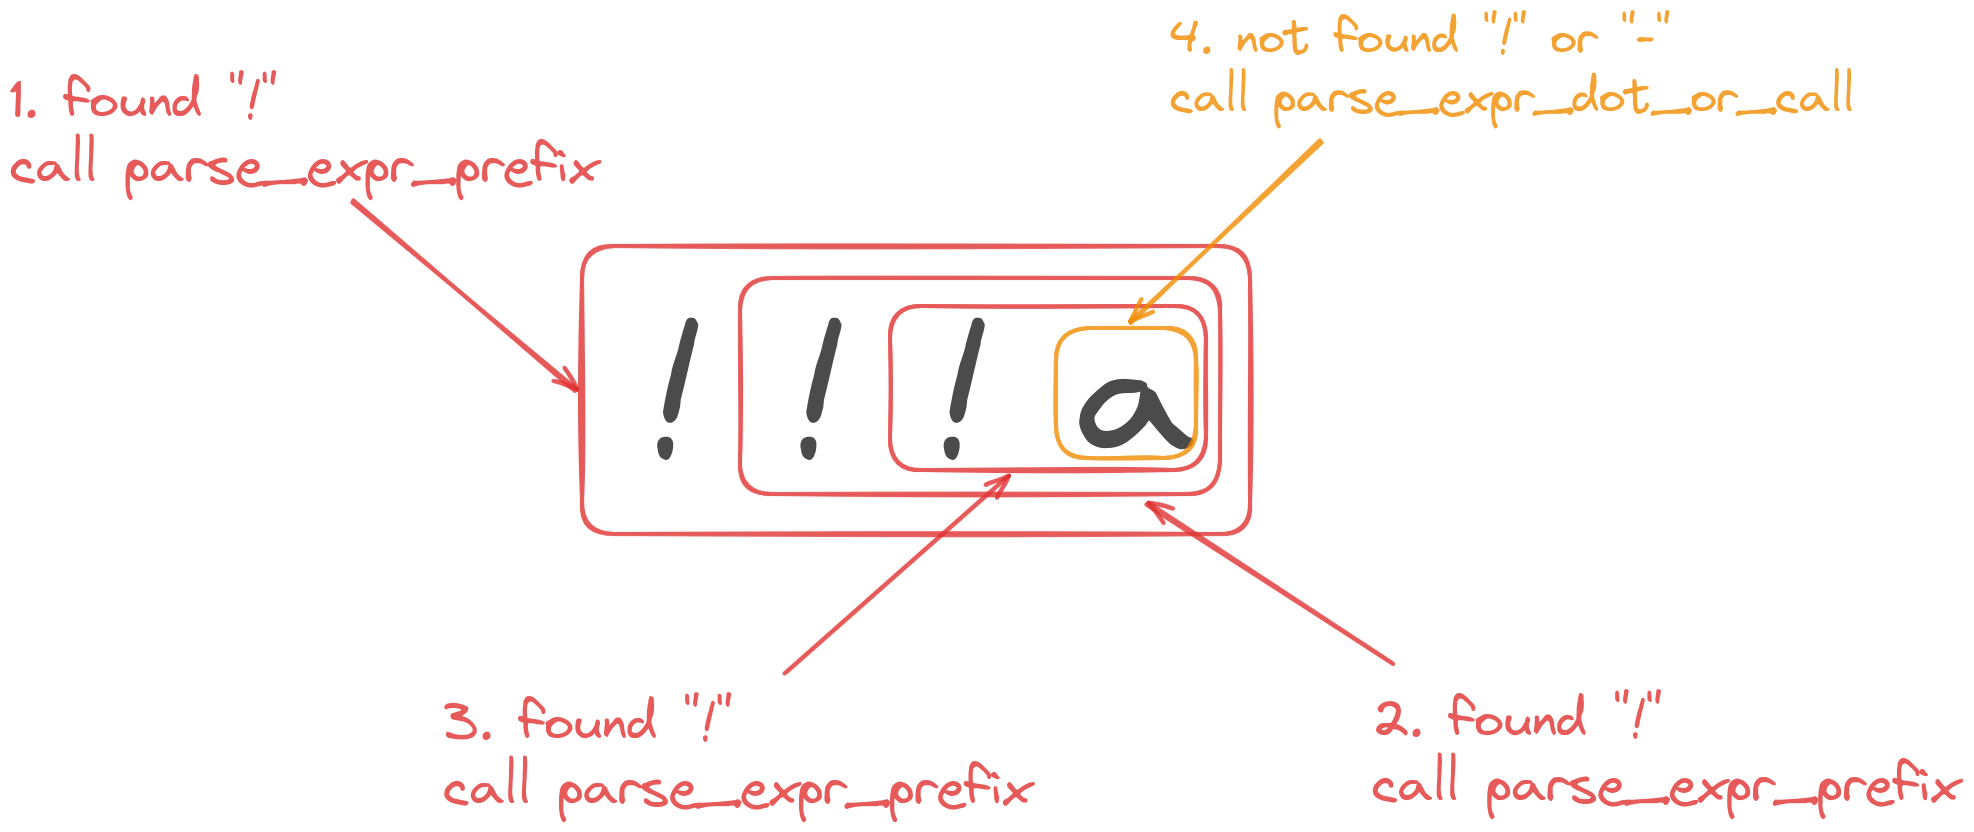
\includegraphics[scale=0.23]{ex-parse-expr-prefix.png}
    \caption{Cách hoạt động của hàm \kw{parse\_expr\_prefix}}
\end{figure}

Giả sử biểu thức cần phân tích là \kw{!!!a}, khi đó, hàm \kw{parse\_expr\_prefix} sẽ phân tích từ tố đầu tiên là \kw{!}, sau đó gọi đệ quy để phân tích phần còn lại của biểu thức. Kết quả trả về sẽ là một biểu thức có toán tử là \kw{Not} và toán hạng là biểu thức \kw{!!a}. Tiếp theo, hàm \kw{parse\_expr\_prefix} sẽ tiếp tục phân tích biểu thức \kw{!!a} và trả về kết quả là một biểu thức có toán tử là \kw{Not} và toán hạng là biểu thức \kw{!a}. Cuối cùng, hàm \kw{parse\_expr\_prefix} sẽ phân tích biểu thức \kw{!a} và trả về kết quả là một biểu thức có toán tử là \kw{Not} và toán hạng là biến \kw{a}. Tới đây, do biểu thức không còn phần tiền tố nên hàm \kw{parse\_expr\_prefix} sẽ gọi tới hàm \kw{parse\_expr\_dot\_or\_call} để phân tích phần biểu thức theo sau. Tiếp theo, ta sẽ phân tích hàm \kw{parse\_expr\_dot\_or\_call} để xem cách thức phân tích phần biểu thức theo sau.

\begin{lstlisting}[]
fn parse_expr_dot_or_call(...) -> PResult<Box<Expr>> {
    let base = self.parse_expr_bottom()?;
    if self.token.is_kind(TokenKind::Dot)
        || self.token.is_open_delim(Delimiter::Parenthesis)
        || self.token.is_open_delim(Delimiter::Bracket)
    {
        self.parse_expr_dot_or_call_with(base)
    } else {
        Ok(base)
    }
}

fn parse_expr_bottom(...) -> PResult<Box<Expr>> {
    match self.token.kind {
        TokenKind::Literal(_) => self.parse_expr_lit(),
        TokenKind::Ident(_, _) => self.parse_expr_ident(),
        TokenKind::OpenDelim(Delimiter::Parenthesis) => {
            self.parse_expr_grouped(Delimiter::Parenthesis)
        }
        TokenKind::OpenDelim(Delimiter::Bracket) => self.parse_expr_array(),
        _ => {
            let err = PError::ExpectedToken {...};
            return Err(vec![err]);
        }
    }
}
\end{lstlisting}

    Hàm \kw{parse\_expr\_dot\_or\_call} gọi tới hàm \kw{parse\_expr\_bottom} để phân tích biểu thức ngay sau phần tiền tố. Hàm \kw{parse\_expr\_bottom} sẽ kiểm tra từ tố hiện tại và phân tích biểu thức dựa trên từ tố đó. Nếu từ tố hiện tại là một giá trị trực tiếp, hàm \kw{parse\_expr\_lit} sẽ được gọi để phân tích giá trị trực tiếp. Nếu từ tố hiện tại là một tên biến, hàm \kw{parse\_expr\_ident} sẽ được gọi để phân tích tên biến. Nếu từ tố hiện tại là kí tự \kw{(}, hàm \kw{parse\_expr\_grouped} sẽ được gọi để phân tích biểu thức trong cặp ngoặc tròn. Nếu từ tố hiện tại là kí tự \kw{[}, hàm \kw{parse\_expr\_array} sẽ được gọi để phân tích biểu thức mảng. Nếu không thỏa mãn trường hợp nào, hàm sẽ báo lỗi. Sau khi có được kết quả phân tích từ tố hiện tại, hàm \kw{parse\_expr\_dot\_or\_call} sẽ kiểm tra từ tố tiếp theo để xác định xem biểu thức tiếp theo có phải là biểu thức truy cập thư viện hay biểu thức gọi hàm không. Nếu từ tố tiếp theo là kí tự \kw{.}, hàm \kw{parse\_expr\_dot} sẽ được gọi để phân tích biểu thức truy cập thư viện. Nếu từ tố tiếp theo là kí tự \kw{(}, hàm \kw{parse\_expr\_call\_with} sẽ được gọi để phân tích biểu thức gọi hàm. Nếu không thỏa mãn trường hợp nào, hàm sẽ báo lỗi. Việc xây dựng như vậy sẽ đảm bảo các phép toán một ngôi hay biểu thức đơn phải được xử lý sau biểu thức có mức ưu tiên cao hơn như biểu thức truy cập thư viện hay biểu thức gọi hàm. Cách xây dựng hàm \kw{parse\_expr\_dot\_or\_call\_with} cũng tương tự như trên.

    Sau khi đã phân tích toàn bộ các biểu thức và toán tử có mức ưu tiên cao: biểu thức truy cập thư viện, biểu thức gọi hàm, biểu thức mảng, biểu thức nhóm, toán tử một ngôi. Trình thông dịch sẽ tiếp tục phân tích các toán tử hai ngôi và xác định thứ tự ưu tiên của các toán tử. Quá trình phân tích này sẽ được thực hiện thông qua hàm \kw{parse\_expr\_rest} như sau:

\begin{lstlisting}[]
fn parse_expr_rest(..., min_prec: usize, mut lhs: Box<Expr>) -> PResult<Box<Expr>> {
    ...
    loop {
        ...
    }

    Ok(lhs)
}
\end{lstlisting}

Hàm này nhận \kw{min\_prec} là mức độ ưu tiên tối thiểu của phép toán hiện tại, \kw{lhs} là biểu thức vế trái. Hàm này sẽ trả về biểu thức nếu hợp lệ, không thì sẽ trả về lỗi. Để tính toán cả biểu thức, ta sẽ tiến hành một vòng lặp. Với mỗi lần lặp, ta sẽ thực hiện các bước sau:

\begin{lstlisting}[]
fn parse_expr_rest(...) -> PResult<Box<Expr>> {
    ...
    loop {
        ...
        let op_assoc = AssocOp::from_token(&self.token);
        if op_assoc.is_none() {
            break;
        }
        let op_assoc = op_assoc.unwrap();
        let prec = op_assoc.precedence();
        if prec < min_prec {
            break;
        }
        ...
        // Special cases:
        if op_assoc == AssocOp::As {
            lhs = self.parse_assoc_op_cast(lhs, lhs_span, ExprKind::Cast)?;
            continue;
        }
        ...
        self.advance();

        let mut rhs = self.parse_expr_prefix()?;
        let fixity = op_assoc.fixity();
        let next_prec = match fixity {
            Fixity::Left => prec + 1,
            Fixity::Right => prec,
        };
        rhs = self.parse_expr_rest(next_prec, rhs)?;
    }
    ...
}
\end{lstlisting}

    Đầu tiên, ta sẽ đọc từ tố hiện tại. Nếu đó không phải là phép toán, tức biểu thức đã kết thúc, ta thoát ra khỏi vòng lặp. Ngược lại, ta sẽ kiểm tra mức độ ưu tiên của phép toán đó thông qua hàm \kw{precedence}. 

\begin{lstlisting}[]
pub fn precedence(...) -> usize {
    ...
    match *self {
        As => 11,
        Multiply | Divide | Modulus => 10,
        Add | Subtract => 9,
        ShiftLeft | ShiftRight => 8,
        BitAnd => 7,
        BitXor => 6,
        BitOr => 5,
        Less | Greater | LessEqual | GreaterEqual | Equal | NotEqual => 4,
        LAnd => 3,
        LOr => 2,
        Assign | AssignOp(_) => 1,
    }
}
\end{lstlisting}

    Như ta có thể thấy, hàm \kw{precedence} sẽ trả về mức độ ưu tiên tương ứng với phép toán đó. Nếu mức độ ưu tiên của phép toán hiện tại thấp hơn so với mức độ ưu tiên tối thiểu (phép toán trước đó) thì ta sẽ không xét nữa. Nếu mức độ ưu tiên Không thấp hơn trước đó, ta sẽ tiến hành phân tích vế phải. Trước đó, ta sẽ kiểm tra thứ tự thực hiện phép tính hiện tại. Nếu thứ tự thực hiện là từ trái qua phải thì phép toán tiếp theo bên vế phải bắt buộc phải có mức ưu tiên lớn hơn thì mới có thể được phép thực hiện trước. Còn nếu chiều thực hiện phép toán từ phải qua trái thì phép toán bên phải không nhất thiết cần mức ưu tiên hơn phép toán hiện tại. Có một trường hợp đặc biệt là khi biểu thức đo là biểu thức ép kiểu. Khi đó chỉ có vế trái cần xét, không có vế phải nên ta có thể trực tiếp xét trường hợp đó rồi kết thúc vòng lặp luôn. Với cách xét như vậy, ta luôn đảm bảo thứ tự thực hiện các phép toán sẽ khớp với mức ưu tiên của chúng.     

    Sau khi đã có đầy đủ thông tin về biểu thức vế trái và biểu thức vế phải, cũng như phép toán của chúng, tùy vào phép toán, ta sẽ phân chúng vào loại biểu thức phù hợp. Chẳng hạn, nếu phép toán là phép cộng, trừ, nhân, chia, ... thì biểu thức gộp của vế trái và vế phải sẽ là một biểu thức nhị phân. Trong khi đó, nếu phép toán là dấu bằng (gán bằng) thì biểu thức thu được sẽ lại là biểu thức gán. Cụ thể, mã nguồn cho việc phân loại biểu thức sẽ như sau:

\begin{lstlisting}[]
fn parse_expr_rest(...) -> PResult<Box<Expr>> {
    ...
    loop {
        ...
        lhs = match op_assoc {
            AssocOp::Add
            | AssocOp::Subtract
            | AssocOp::Multiply
            | AssocOp::Divide
            | AssocOp::Modulus
            | AssocOp::LAnd
            | AssocOp::LOr
            | AssocOp::BitXor
            | AssocOp::BitAnd
            | AssocOp::BitOr
            | AssocOp::ShiftLeft
            | AssocOp::ShiftRight
            | AssocOp::Equal
            | AssocOp::Less
            | AssocOp::LessEqual
            | AssocOp::NotEqual
            | AssocOp::Greater
            | AssocOp::GreaterEqual => {
                ...
                let binary = self.mk_binary(...);
                self.mk_expr(binary, ...)
            }
            AssocOp::Assign => self.mk_expr(...),
            AssocOp::AssignOp(k) => {
                let aop = match k {
                    BinOpToken::Plus => BinOpKind::Add,
                    BinOpToken::Minus => BinOpKind::Sub,
                    BinOpToken::Star => BinOpKind::Mul,
                    BinOpToken::Slash => BinOpKind::Div,
                    BinOpToken::Percent => BinOpKind::Mod,
                    BinOpToken::Caret => BinOpKind::BitXor,
                    BinOpToken::And => BinOpKind::BitAnd,
                    BinOpToken::Or => BinOpKind::BitOr,
                    BinOpToken::Shl => BinOpKind::Shl,
                    BinOpToken::Shr => BinOpKind::Shr,
                };
                let aopexpr = self.mk_assign_op(...);
                self.mk_expr(aopexpr, ...)
            }
            AssocOp::As => unreachable!("AssocOp::As should be handled separately"),
    }
    ...
}
\end{lstlisting}

    Để hiểu rõ hơn về cách thức hoạt động của hàm trên, ta sẽ xem xét một ví dụ đơn giản sau đây:

\begin{figure}[H]
    \centering
    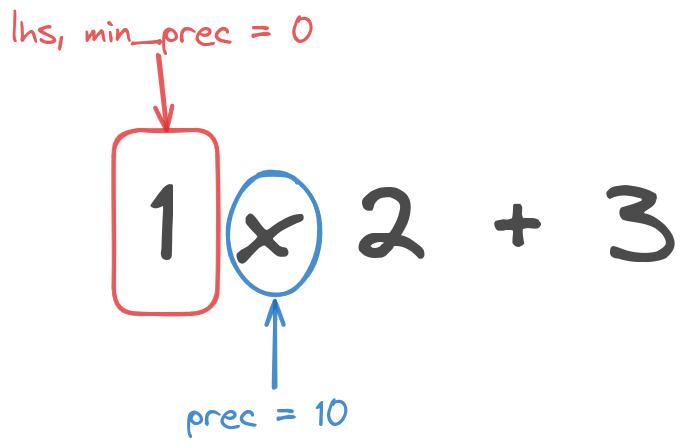
\includegraphics[scale=0.4]{ex-expr-rest-1.png}
    \caption{Ví dụ cách phân tích cú pháp biểu thức 1}
\end{figure}

Cho một biểu thức đơn giản: \kw{1 * 2 + 3}, sau khi xét xong tiền tố (như đã miêu tả ở phần trên), ta sẽ có vế trái đầu tiên là số \kw{1}. Đây là biểu thức đầu tiên nên mức độ ưu tiên tối thiểu yêu cầu sẽ là \kw{0}. Phép toán đọc được hiện tại là \kw{*} có mức độ ưu tiên là \kw{10} lớn hơn \kw{0}, nên ta sẽ xét tiếp vế phải. Do phép toán nhân thì sẽ thực hiện từ trái qua phải, nên phép toán tiếp theo của vế phải cần một mức độ ưu tiên tối thiểu là \kw{11} để được thực hiện trước.

\begin{figure}[H]
    \centering
    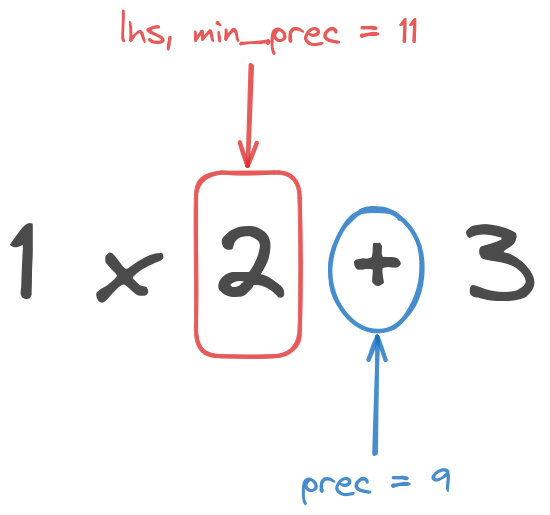
\includegraphics[scale=0.4]{ex-expr-rest-2.png}
    \caption{Ví dụ cách phân tích cú pháp biểu thức 2}
\end{figure}

    Tương tự như phía trên, ta sẽ thu được biểu thức vế trái lúc này là số \kw{2}, nhưng để thực hiện được phép toán, phép toán yêu cầu cần mức độ ưu tiên tối thiểu là \kw{11}. Tuy nhiên, ký hiệu toán học đọc được lần này là dấu \kw{+} với mức độ ưu tiên là \kw{9}, tức thấp hơn so với yêu cầu. Vì thế, ta sẽ kết thúc việc xét vòng lặp và trả về biểu thức vế trái, tức là biểu thức \kw{2}.

\begin{figure}[H]
    \centering
    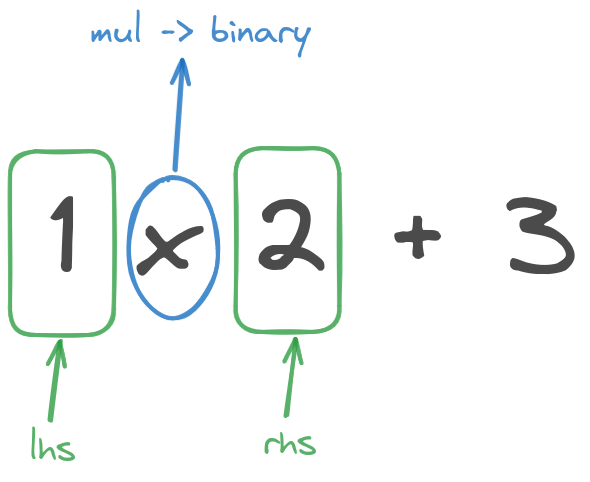
\includegraphics[scale=0.4]{ex-expr-rest-3.png}
    \caption{Ví dụ cách phân tích cú pháp biểu thức 3}
\end{figure}

    Quay trở lại hàm cũ, như vậy ta vừa tính được vế phải là số \kw{2}, vế trái tính được trước khi gọi đệ quy là \kw{1}, và phép toán là phép nhân. Như vậy, biểu thức tạo ra được là biểu thức nhị phân với thông tin vế trái, vế phải, phép toán như vừa nêu. Ta sẽ gán biểu thức này cho vế trái và tiếp tục vòng lặp.

\begin{figure}[H]
    \centering
    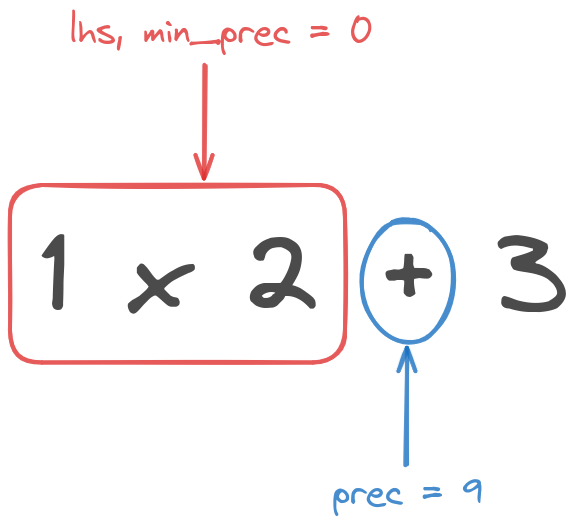
\includegraphics[scale=0.4]{ex-expr-rest-4.png}
    \caption{Ví dụ cách phân tích cú pháp biểu thức 4}
\end{figure}

    Bây giờ, vế trái lại là biểu thức \kw{1 * 2}, với mức ưu tiên tối thiểu cần đạt được là \kw{0}, phép toán hiện tại đọc được là dấu cộng, mức độ ưu tiên là \kw{9}. Ta lại tiến hành xét vế phải với mức ưu tiên tối thiểu là \kw{10} (do phép cộng cần thực hiện từ trái qua phải). 

\begin{figure}[H]
    \centering
    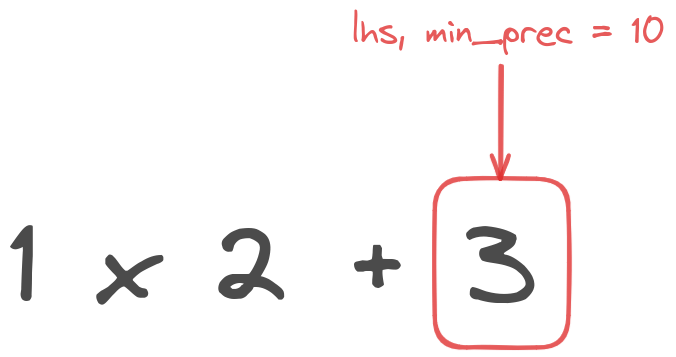
\includegraphics[scale=0.4]{ex-expr-rest-5.png}
    \caption{Ví dụ cách phân tích cú pháp biểu thức 5}
\end{figure}

    Tiếp tục xét, vế trái tại lần gọi hiện tại là số \kw{3}. Do không còn phép toán nên ta lại kết thúc vòng lặp và trả về biểu thức là \kw{3}. 

\begin{figure}[H]
    \centering
    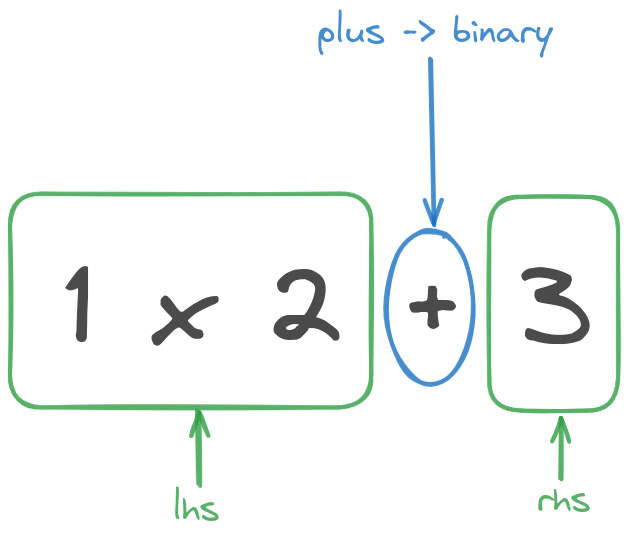
\includegraphics[scale=0.4]{ex-expr-rest-6.png}
    \caption{Ví dụ cách phân tích cú pháp biểu thức 6}
\end{figure}

    Biểu thức vế trái hiện tại giờ là \kw{1 * 2}, vế phải là \kw{3}, phép toán là phép cộng. Kết quả sẽ cho ra biểu thức nhị phân \kw{1 * 2 + 3} và gán vào biểu thức vế trái.

\begin{figure}[H]
    \centering
    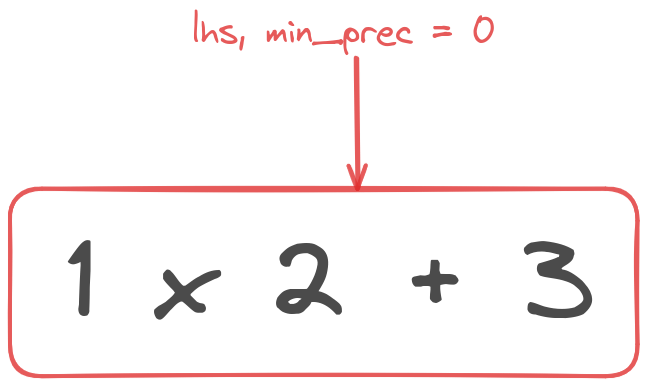
\includegraphics[scale=0.4]{ex-expr-rest-7.png}
    \caption{Ví dụ cách phân tích cú pháp biểu thức 7}
\end{figure}

    Cuối cùng, biểu thức vế trái hiện tại là cả \kw{1 * 2 + 3}. Ta không đọc được phép toán nào nữa, tiến hành trả về biểu thức vế trái hiện tại, kết thúc quá trình phân tích cú pháp biểu thức. Và đây sẽ là kết quả thu được của quá trình trên:

\begin{figure}[H]
    \centering
    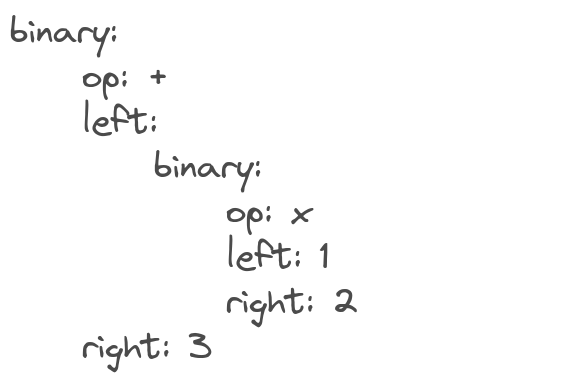
\includegraphics[scale=0.6]{ex-expr-rest-8.png}
    \caption{Ví dụ cách phân tích cú pháp biểu thức 8}
\end{figure}

    Tuy được xây dựng phức tạp, nhưng cách xây dựng này sẽ giúp cho việc mở rộng loại biểu thức cực kì dễ dàng. Nếu bất cứ khi nào ta muốn thêm một phép toán mới, ta chỉ cần bổ sung chúng vào danh sách thứ tự mức ưu tiên trong hàm \kw{precedence}, cũng như trong hàm \kw{parse\_expr\_rest}. Như vậy, ta đã xây dựng xong toàn bộ bộ phân tích cú pháp. Tiếp theo, ta sẽ tới một bộ xử lý cũng vô cùng quan trọng, đó chính là bộ phân tích ngữ nghĩa.
